\chapter{Appendix}
\appendix

\section{Corpus Text Legnth Statistics }
\begin{longtable}{lllll}
\caption{Statistics on Average Text Length by Task and JLPT Proficiency Level}\label{tab:text_len}\\

\toprule
\textbf{JLPT} & \textbf{Writing Task} & \textbf{Avg. Len} & {std} & \textbf{\# of Texts}\\
\midrule
\endfirsthead

\toprule
\textbf{JLPT} & \textbf{Writing Task} & \textbf{Avg. Len} & {std} & \text{\# of Texts}\\
\midrule
\endhead

\midrule
\multicolumn{5}{r}{{Continued on next page}}\\
\midrule
\endfoot

\bottomrule
\endlastfoot


N5	&   SW1	&   91.61	&   33.32	&   176\\
N5	&   SW2	&   99.69	&   37.77	&   176\\
N5	&   e	&   333.83	&   89.82	&   95\\
N5	&   m1	&   133.69	&   52.21	&   96\\
N5	&   m2	&   125.55	&   45.01	&   96\\
N5	&   m3	&   123.40	&   50.90	&   96\\
N4	&   SW1	&   105.51	&   33.92	&   318\\
N4	&   SW2	&   115.47	&   38.73	&   318\\
N4	&   e	&   379.20	&   106.04	&   199\\
N4	&   m1	&   152.04	&   55.15	&   199\\
N4	&   m2	&   150.82	&   55.26	&   199\\
N4	&   m3	&   145.74	&   54.03	&   198\\
N3	&   SW1	&   114.88	&   36.28	&   297\\
N3	&   SW2	&   119.15	&   38.93	&   297\\
N3	&   e	&   396.86	&   99.35	&   187\\
N3	&   m1	&   165.89	&   66.51	&   187\\
N3	&   m2	&   157.24	&   50.79	&   187\\
N3	&   m3	&   152.98	&   55.38	&   187\\
N2	&   SW1	&   132.25	&   44.81	&   165\\
N2	&   SW2	&   136.19	&   45.20	&   165\\
N2	&   e	&   422.38	&   100.96	& 120\\
N2	&   m1	&   189.41	&   67.79	&   122\\
N2	&   m2	&   184.93	&   71.51	&   122\\
N2	&   m3	&   173.65	&   69.05	&   122\\
N1	&   SW1	&   120.27	&   35.88	&   44\\
N1	&   SW2	&   132.30	&   45.65	&   44\\
N1	&   e	&   396.65	&   110.20	&   34\\
N1	&   m1	&   200.12	&   69.94	&   34\\
N1	&   m2	&   212.62	&   79.85	&   34\\
N1	&   m3	&   182.53	&   66.88	&   34\\
NS	&   SW1	&   114.38	&   30.41	&   50\\
NS	&   SW2	&   129.52	&   36.49	&   50\\
NS	&   e	&   399.67	&   66.51	&   48\\
NS	&   m1	&   167.60	&   51.12	&   48\\
NS	&   m2	&   144.27	&   59.16	&   48\\
NS	&   m3	&   170.25	&   67.43	&   48\\

\end{longtable}

\section{Story Telling Task Images (SW1, SW2)}
\begin{figure}[h!]
    \centering
    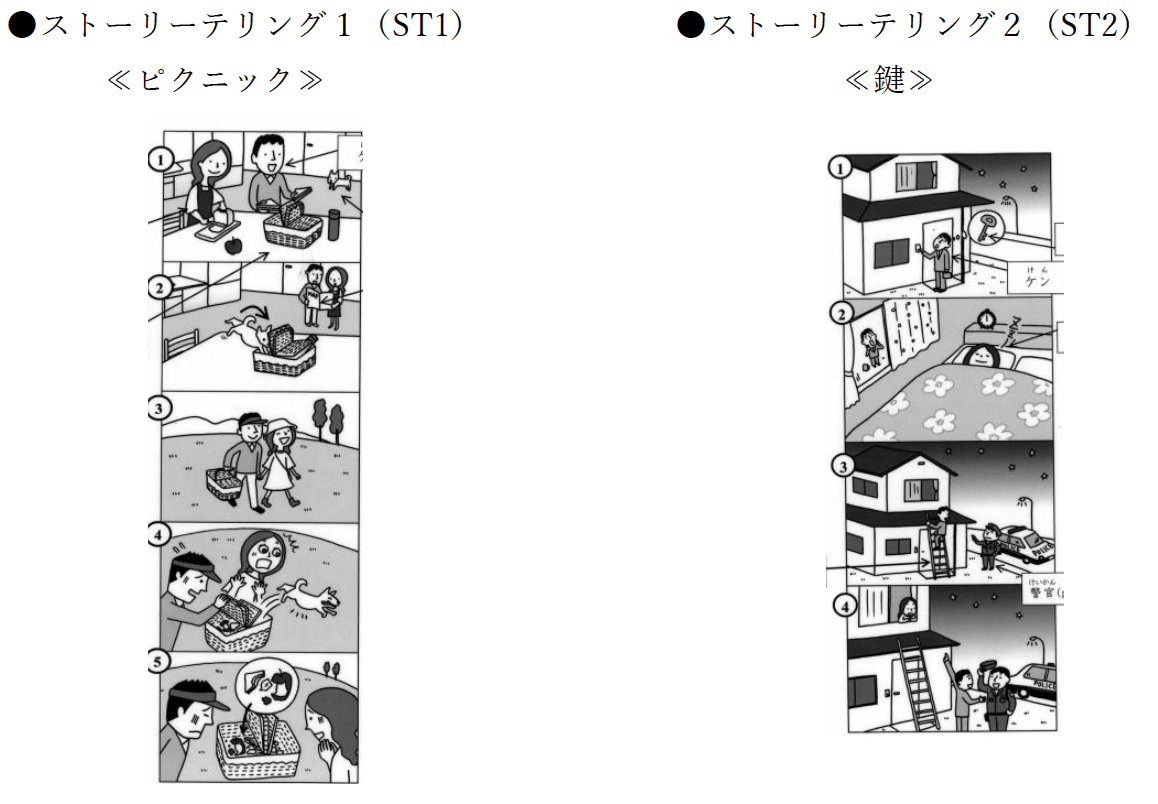
\includegraphics[scale=.45]{img/ST.png}
    \caption[Story Telling Tasks]{Images used for the two story-telling tasks. Learners were instructed to construct a narrative based on these visual prompts. }
    \label{fig:ST}
\end{figure}


\section{Complexity Features}
Below is are table detailing the complexity measures calculated from each domain.

\usepackage{array}
\usepackage{longtable}
\usepackage{multirow}

\begin{longtable}{>{\raggedright\arraybackslash}p{4cm} p{10cm}}
\caption{Overview of Complexity Features} \label{tab:complexity-measures} \\
\hline
\textbf{Domain} & \textbf{Measure} \\
\hline
\endfirsthead

\multicolumn{2}{c}%
{\tablename\ \thetable\ -- \textit{continued from previous page}} \\
\hline
\textbf{Domain} & \textbf{Measure} \\
\hline
\endhead

\hline \multicolumn{2}{r}{\textit{Continued on next page}} \\
\endfoot

\hline
\endlastfoot

\multirow{10}{=}{\textbf{Syntactic Complexity}}
& Sentence Length \\
& Clause Length \\
& Clauses per Sentence \\
& Coordinate Clauses per Sentence \\
& Coordinate Clauses Ratio to All Clauses \\
& Subordinate Clauses per Sentence \\
& Subordinate Clauses Ratio to All Clauses \\
& Subordinate to Coordinating Clause Ratio \\
& Average Noun Phrase Length \\
& Average Verb Phrase Length \\

\multirow{7}{=}{\textbf{Lexical Complexity}}
& Corrected Type-Token Ratio (CTTR) \\
& Noun Density \\
& Verb Density \\
& Adjective Density \\
& Adverb Density \\
& Measure of Textual Lexical Diversity (MTLD) \\
& Lexical Frequency Profile (LFP) \\

\multirow{3}{=}{\textbf{Morphological Complexity}}
& MCI-5 (Morphological Complexity Index – surface form) \\
& MCI-10 (Morphological Complexity Index – inflectional form) \\
& Japanese Morphological Richness Analyzer(JMRA) – MATTR\\
&Japanese Morphological Richness Analyzer(JMRA) - MTLD \\

\end{longtable}



\section{Criterial Features}
\begin{longtable}{p{2cm} p{4cm} p{8cm}}
\caption{Grammar Forms extracted as criterial features from the learner texts.
\label{tab:Criterial-Features}}\\
\toprule
\textbf{JLPT Level} & \textbf{Grammar Form} & \textbf{English Equivalent}  \\
\midrule
\endfirsthead

\toprule
\textbf{JLPT Level} & \textbf{Grammar Form} & \textbf{English Equivalent}\\
\midrule
\endhead

\midrule \multicolumn{3}{r}{{Continued on next page}}\\
\midrule
\endfoot

\bottomrule
\endlastfoot

N1  &	あえて &	        dare to \\
N1  &	案の定 &	        just as one thought\\
N1  &	あらかじめ   &	beforehand; in advance\\
N1  &	ばこそ &	        only because\\
N1  &	どうにも○○ない    &	not … by any means\\
N1  &	ほうがましだ  &	I would rather\\
N1  &	いかなる	&       any kind of\\
N1	&   可能性がある  &	there's a possibility\\
N1	&   かつて	&       once; before\\
N1	&   嫌いがある &     	to have a tendency to\\
N1	&   きりがない	&   there's no end to\\
N1	&   もしくは	    &   or; otherwise\\
N1	&   てみせる	    &   I'll definitely\\
N1	&   てしかるべきだ & 	should\\
N1	&   という     &   	all; every\\
N1	&   とは	    &       (indicates word or phrase being defined); or expression of surprisal\\
N1  &	とはいえ	&       nonetheless; although\\
N4	&   以上  	&       over\\
N2	&   以上に	&       more than; no less than\\
N2	&   えない    &     	unable to; cannot\\
N2	&   える / うる &	can; is possible\\
N2	&   お○○願う &     	could you please\\
N2	&   恐れがある &     	there are fears that\\
N2	&   かいがある &     	it's worth one's effort to do something\\
N2	&   限り	        &   as long as; while… is the case\\
N2	&   かと思ったら / かと思うと	& then again; just when; no sooner than\\
N2	&   から言うと   &	in terms of; from the point of view of\\
N2	&   からして	&   judging from; based on\\
N2	&   からすると / からすれば	&   judging from; considering\\
N3	&   さらに    &   	furthermore; again; more and more\\
N2	&   しかも	&       moreover; furthermore\\
N2	&   次第	     &      as soon as\\
N2	&   次第だ / 次第で &	depending on; so\\
N2	&   その上	&       besides; in addition; furthermore\\
N3	&   それとも  &	    or; or else\\
N2	&   それにしても & 	nevertheless; even so\\
N3	&   だけでなく   &	not only… but also\\
N2	&   つつ	&           while; although\\
N3	&   つもりで	&       with the intention of doing\\
N2	&   でしかない	&   merely; nothing but; no more than\\
N3	&   てしょうがない & 	very; extremely\\
N2	&   てたまらない	&   very; extremely; can't help but do\\
N2	&   て当然だ	&       natural; as a matter of course\\
N2	&   てはいられない & 	can't afford to; unable to\\
N2	&   というものだ  &	something like…; something called…\\
N2	&   と考えられる &	one can think that…\\
N3	&   ないことにはない &	states something is not quite impossible but requires great effort\\
N2	&   ないではいられない & can't help but feel; can't help but do\\
N2	&   なお	    &        furthermore; still; yet (used to add more information to the )\\
N2	&   にかかわらず &	regardless of\\
N2	&   に限って &	    only; particularly when\\
N2	&   に限らず &	    not just; not only… but also\\
N2	&   に限る &       	nothing better than; there's nothing like\\
N2	&   に決まっている &	I'm sure that…\\
N2	&   に応えて	    &   in response to\\
N2	&   に基づいて   &   	based on\\
N2	&   に過ぎない	&   no more than; just; merely\\
N2	&   にもかかわらず &	despite; in spite of; although\\
N2	&   ねばならない  &	have to; must\\
N2	&   果たして    &  	sure enough; really\\
N2	&   ふうに	&       in a way (this way/that way/what way)\\
N3	&   ぶりに	&       for the first time in\\
N3	&   むしろ	&       rather; instead\\
N2	&   もかまわず   &	without worrying about\\
N2	&   もっとも    &	but then; although\\
N2	&   ものがある &     	(sentence-ending expression of strong judgement)\\
N2	&   ものだから   &	because; the reason is\\
N2	&   ものの      &   	but; although\\
N2	&   やがて &       	soon; before long; eventually\\
N2	&   やら○○やら  &	such things as\\
N2	&   よりほかない  &	to have no choice but\\
N3	&   あまり     &   	so much… that \\
N3	&   あまりに    &	so much… that; too…\\
N3	&   いくら○○ても / いくら○○でも   &	no matter how\\
N3	&   一方だ	    &   more and more; continue to \\
N2	&   一方で	&   on one hand; on the other hand \\
N3	&   うちに &   	while; before; doing \\
N3	&   おかげで &	thanks to; because of \\
N3	&   がたい &   	hard to; difficult to\\
N3	&   ぎみ  &   	-like; -looking\\
N3	&   きる  &	    to do something completely\\
N3	&   切れない	 &  being too much to finish\\
N3	&   くせに &   	even though; and yet; despite\\
N3	&   決して○○ない &	never; by no means \\
N3	&   こそ	    &   certainly (emphasises the previous word)\\
N4	&   ことがある   &	can; sometimes happens\\
N3	&   ことはない   &	there is no need to; never happens\\
N3	&   さえ	    &   even  \\
N3	&   しかない    &	have no choice but\\
N3	&   ずに  &   	without (doing) \\
N3	&   せいで &   	because of  \\
N3	&   だけど &   	but; however\\
N3	&   確かに &	    surely; certainly\\
N3	&   たびに &   	everytime; whenever\\
N3	&   ついでに   &	taking the opportunity; while (you) are at it\\
N3	&   っぱなし  &	    leaving something still in use\\
N3	&   っぽい &   	    -ish; -like \\
N3	&   つまり &   	    in other words; that is to say\\
N4	&   という &   	    called; named\\
N3	&   というより  &    rather than\\
N3	&   と共に &   	    together with\\
N3	&   とは限らない &	not necessarily so; is not always true\\
N3	&   ながら / いながら / ながらも	&   although; despite \\
N3	&   なぜなら / なぜかというと  &	because; the reason is\\
N3	&   なるべく    &	as much as possible\\
N3	&   に比べて	&       compared to\\
N3	&   に違いない   &	I'm sure; no doubt that\\
N3	&   ばよかった   &	should have; it would have been better if\\
N3	&   べき       &   	must do; should do\\
N3	&   ほど	    &       the more; to the extent that; so much… that\\
N3	&   もしかしたら  &	perhaps; maybe\\
N3	&   ような気がする &	have a feeling that; think that\\
N4	&   受身形 &        Passive Form\\
N4	&   あまり○○ない &	not very; not much\\
N4	&   かしら &       	I wonder\\
N4	&   がする &       	smell; hear; taste\\
N4	&   かもしれない  &	might; maybe\\
N4	&   ございます   &	there is (honorific ある)\\
N4	&   させられる   &	to be made to do something\\
N4	&   させる &       	to make/let somebody do something\\
N4	&   しか○○ない &	    only; nothing but\\
N5	&   すぎる     &   	too much\\
N4	&   たところ    &   	just finished doing; was just doing\\
N4	&   たばかり    &   	just did; something just happened\\
N4	&   たら  &       	if; after; when\\
N4	&   たらどう    &	why don't you\\
N5	&   たり○○たり  &	do such things like\\
N4	&   ていただけませんか&	could you please\\
N4	&   ているところ  &	in the process of doing\\
N4	&   てくれる    &	to do something for someone \\
N4	&   てしまう / ちゃう  &	to do something (regretfully); to do something (completely) \\
N4	&   てすみません  &	I'm sorry for\\
N4	&   てもらう    &	to get somebody to do something\\
N4	&   と思う &       	I think; you think\\
N4	&   ところ     &   	about to; on the verge of\\
N5	&   なくてはいけない / なくてはならない &	must do; have to do\\
N4	&   なさい	&       order somebody to do something\\
N4	&   なさる &       	to do (honorific する) \\
N4	&   にくい     &   	difficult to\\
N4	&   のように / のような &	like; similar to\\
N4	&   みたい &       	like; similar to; resembling\\
N4	&   みたいに/みたいな   &	like; similar to\\
N4	&   やすい &       	easy to; likely to\\
N4	&   ようだ &       	it seems that; it appears that; it looks like\\
N4  &	より  &       	than\\
N4	&   られる1    &   	to be able to do something\\
N4	&   られる2    &   	to do (by someone) (passive 受身形)\\
N5	&   いちばん    &	the most \\
N3	&   くらい / ぐらい   &	about; approximately\\
N5	&   たい  &	want to\\
N5	&   つもり &	plan to; intend to\\
N5	&   てください   &	please do…\\
N5	&   ほうがいい   &	it'd be better to, state a preference\\
N5	&   ほうがいい2  &   	it'd be better to not\\

\end{longtable}

\section{EBM Top 30 Features Rank}

\begin{longtable}{p{2cm} p{4cm} p{8cm}}
\caption{The top 30 features ranked by importance
\label{tab:top30-importance}}\\
\toprule
\textbf{Rank} & \textbf{Feature/Grammar Form} & \textbf{score}  \\
\midrule
\endfirsthead

\toprule
\textbf{Rank} & \textbf{Feature/Grammar Form} & \textbf{score}\\
\midrule
\endhead

\midrule \multicolumn{3}{r}{{Continued on next page}}\\
\midrule
\endfoot

\bottomrule
\endlastfoot

1& Coordinate Clauses per sentence & 0.06319425574144552\\
2& Coordinate Clauses per clause & 0.05830217807245611\\
3& JLPT Vocab percent N2 & 0.05471817016904914\\
4& Mean Hierarchical Distance (MHD) & 0.05396135139120442\\
5& SCfreq& 0.049155282937905664\\
6& mci\_5\_surface& 0.044248016414937565\\
7& mci\_10\_surface& 0.043724866017562855\\
8& JLPT Vocab percent N4& 0.03720183898303819\\
9& Avg Clause per Sent& 0.036563372305653305\\
10& LFP\_OOV\_percent& 0.03576892451595661\\
11& Avg Sent Length& 0.03150024426332492\\
12& CF\_ukemi\_N4\_ratio& 0.031040424071531028\\
13& mci\_10\_inflection& 0.030583392734263356\\
14& JMRA\_all\_MATTR& 0.030315194949040766\\
15& JMRA\_function\_MATTR& 0.03029683172245733\\
16& MDD& 0.028525340600706835\\
17& adverb\_density& 0.028088917437378968\\
18& adjective\_density& 0.027803958533299335\\
19& JMRA\_aux\_chains& 0.02701872734587644\\
20& Subordinate Clauses per clause& 0.02622726570177418\\
21& JLPT Vocab N2& 0.026195347995648457\\
22& LFP\_3k\_percent& 0.025533909411994203\\
23& verb\_density& 0.024132688274859506\\
24& LFP\_4k\_percent& 0.023979708988820472\\
25& LFP\_9k\_percent& 0.023559193367060326\\
26& JLPT Vocab percent N5& 0.02312553126140337\\
27& JMRA\_content\_MTLD& 0.022763280338891856\\
28& CF\_tekuru\_N4\_ratio& 0.022705446651666256\\
29& LFP\_6k\_percent& 0.02260014100511992\\
30& JLPT Vocab percent N1& 0.022057944526285695 \\

\end{longtable}
